This chapter explains the experiments we performed and the results we obtained in Visual Spatial Reasoning.

\section{Models} \label{sec:vsr_models}

We introduce baseline models and our models.

\paragraph{Baselines.} VSR authors \cite{liu2022visual} test three popular VLMs: VisualBERT \cite{li2019visualbert}, 
LXMERT \cite{tan2020lxmert}, and
ViLT \cite{kim2021vilt}. All three models are stacked Transformers \cite{vaswani2017attention} that take image and text pairs as input. The difference mainly lies in how or whether they encode position information of objects. Checkpoints are saved every 100 iterations and the best checkpoint on the dev set is used for testing. All models are run three times using three random seeds.

\paragraph{Ours.} We first test the same baseline models. We also evaluate a ViLT model that has only been finetuned on NLVR2. We evaluate BLIP \cite{li2022blip} trained on VSR and NLVR2.

\section{Results} \label{sec:vsr_results}

\subsection{Compared To Humans}

\paragraph{Baseline}

See \cref{tab:vsr_results_base}. The gap between dev and tests becomes much greater on zero-shot split likely due to the smaller size of both dev and test sets.

\begin{table}[ht]
\centering
%\setlength{\tabcolsep}{2.8pt}
\small
\begin{tabular}{lcccccc}
\toprule
& \multicolumn{2}{c}{random split} &  & \multicolumn{2}{c}{zero-shot split} \\
\cmidrule(l){2-3} 	\cmidrule(l){4-6}
model$\downarrow$ & dev & test & & dev & test  \\
\midrule
human & \multicolumn{5}{c}{95.4}   \\
\midrule
VisualBERT & 59.2$_{\pm0.9}$ & 57.4$_{\pm0.9}$ & & 57.4$_{\pm2.2}$  & 54.0$_{\pm1.3}$  \\ 
LXMERT & \textbf{73.8}$_{\pm1.2}$  & \textbf{72.5}$_{\pm1.4}$ & & \textbf{69.2}$_{\pm1.0}$  & \textbf{63.2}$_{\pm1.7}$  \\ 
ViLT & 71.9$_{\pm1.3}$  & 71.0$_{\pm0.7}$  & & 66.7$_{\pm1.7}$  & 62.4$_{\pm1.5}$ \\ 
\bottomrule
\end{tabular}
\caption{Model performance on VSR. Results of both random and zero-shot splits, both validation and tests are listed.}
\label{tab:vsr_results_base}
\end{table}

\paragraph{Ours}

\subsection{Results By Relation}

\paragraph{Baseline}

See \cref{fig:performance_by_rel_base}

\begin{figure*}
    \centering
\begin{subfigure}[b]{\linewidth}
    \centering
    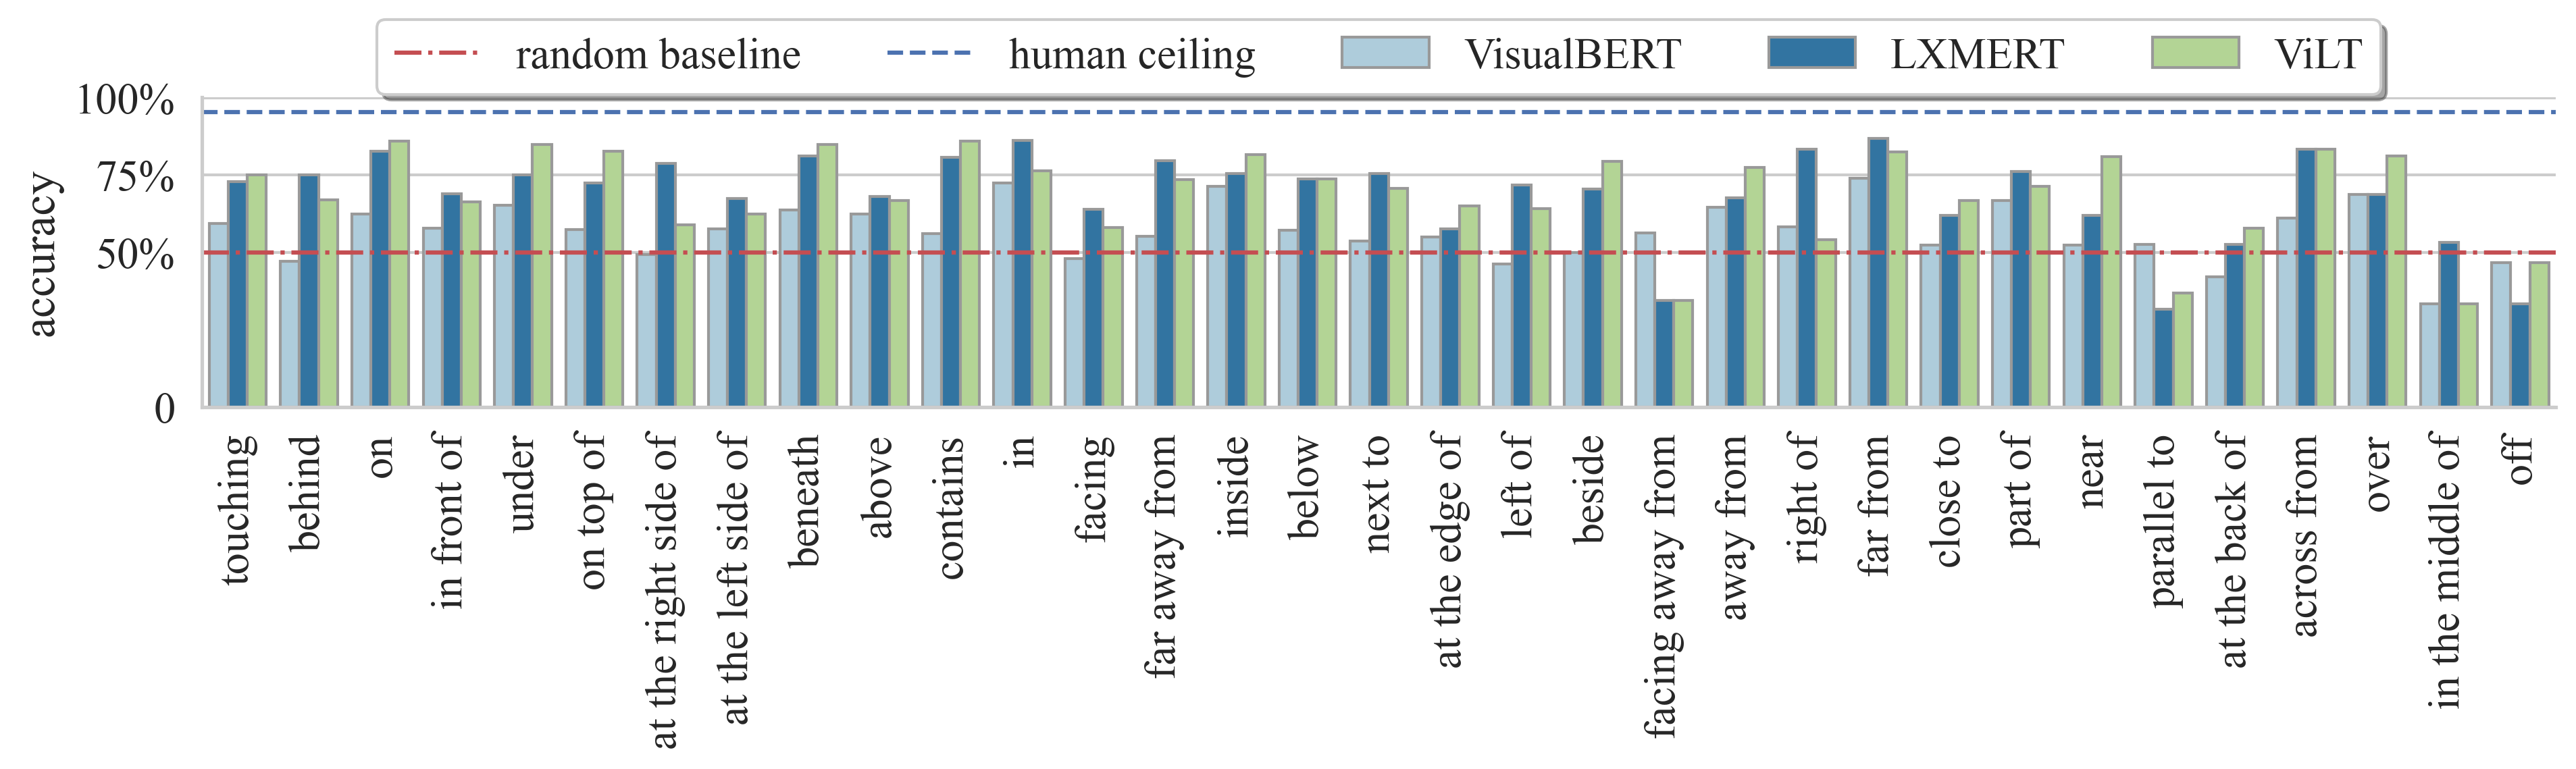
\includegraphics[width=\linewidth]{images/visual-spatial-reasoning/performance_by_relation_random_split_v2.png}
    \vspace{-1cm}
    \caption{random split}
\end{subfigure}
\begin{subfigure}[b]{\linewidth}
    \centering
    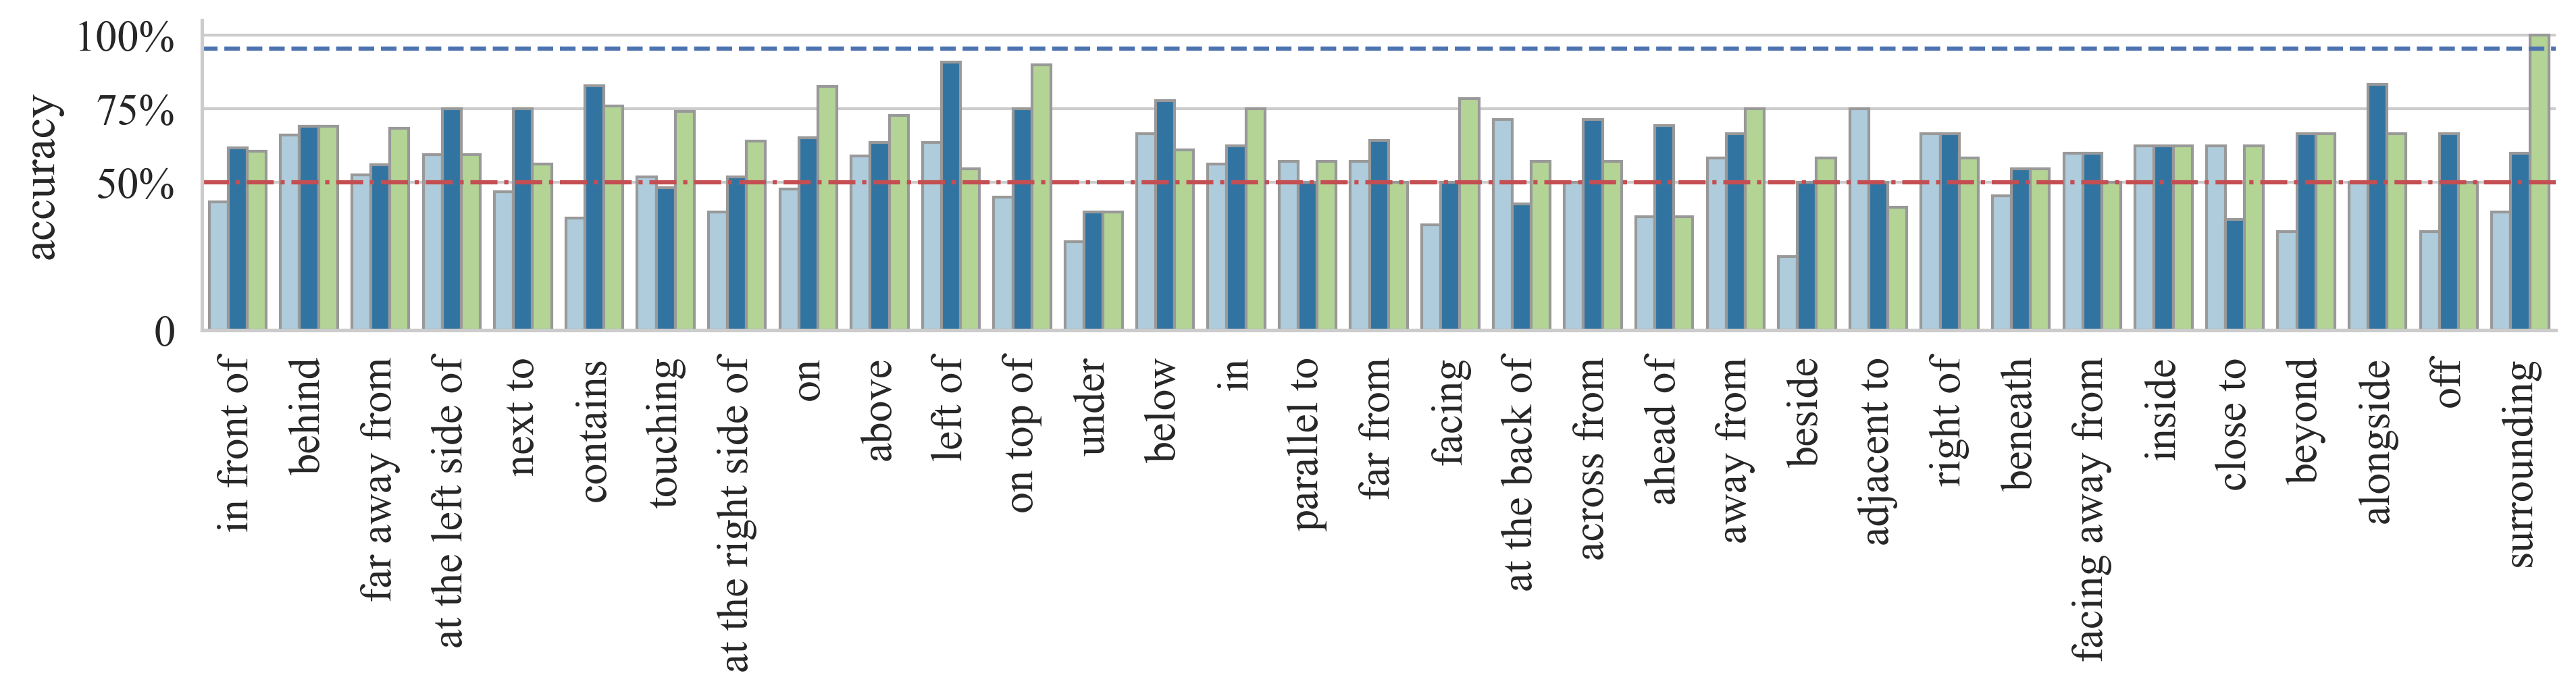
\includegraphics[width=\linewidth]{images/visual-spatial-reasoning/performance_by_relation_zeroshot_split_v2.png}
    \vspace{-1cm}
    \caption{zero-shot split}
\end{subfigure}
\caption{Performance by relation on the random (upper) and zero-shot (lower) split test sets. Relation order sorted by frequency (high to low from left to right). Only relations with more than 15 and 5 occurrences on the random and zero-shot tests respectively are shown. }
    \label{fig:performance_by_rel_base}
\end{figure*}

\paragraph{Ours}

See \cref{fig:performance_by_rel}

\begin{figure}[ht]
    \centering
\begin{subfigure}[b]{\linewidth}
    \centering
    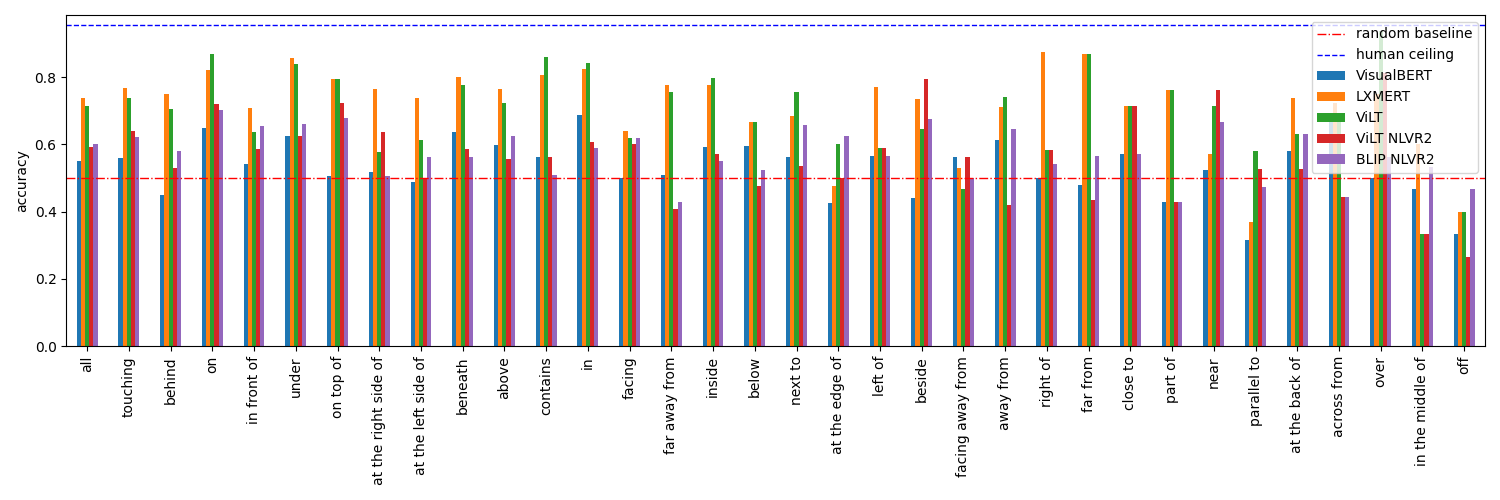
\includegraphics[width=\linewidth]{images/visual-spatial-reasoning/performance_rel_random.png}
    \vspace{-1cm}
    \caption{random split}
\end{subfigure}
\begin{subfigure}[b]{\linewidth}
    \centering
    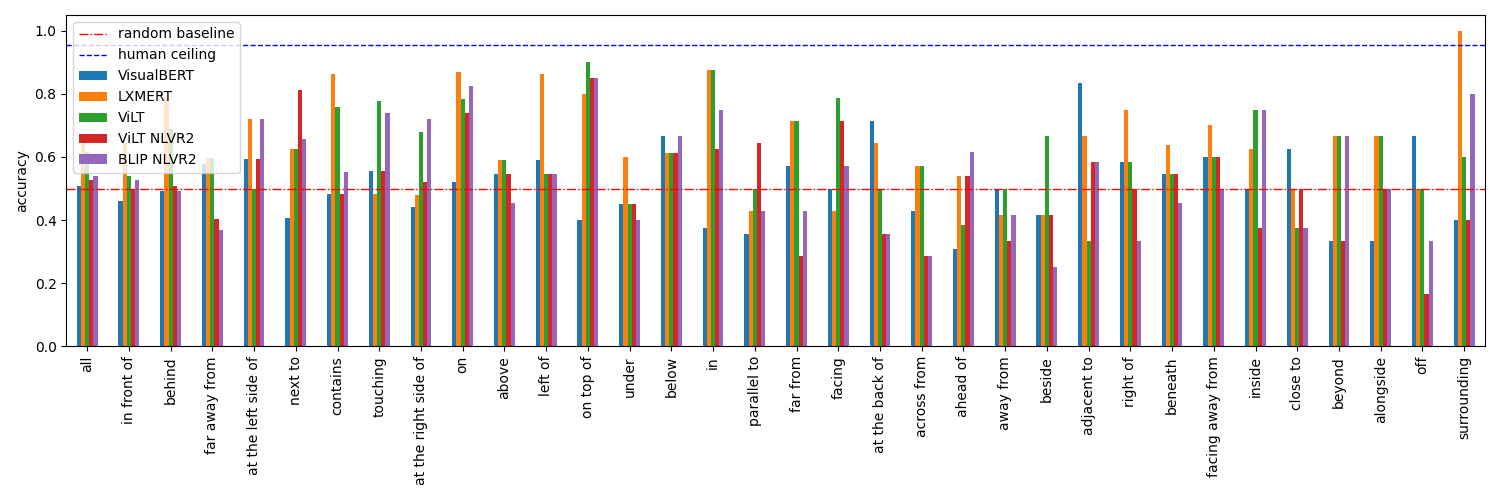
\includegraphics[width=\linewidth]{images/visual-spatial-reasoning/performance_rel_zeroshot.png}
    \vspace{-1cm}
    \caption{zero-shot split}
\end{subfigure}
\caption{Performance by relation on the random (upper) and zero-shot (lower) split test sets. Relation order sorted by frequency (high to low from left to right). Only relations with more than 15 and 5 occurrences on the random and zero-shot tests respectively are shown. }
    \label{fig:performance_by_rel}
\end{figure}

See \cref{tab:results-by-relation-random} and \cref{tab:results-by-relation-zeroshot}

\begin{table}[ht]
\centering
\begin{tabular}{lrrrrrr}
\toprule
relation &  number &  VisualBERT &  LXMERT &  ViLT &  ViLT NLVR2 &  BLIP NLVR2 \\
\midrule
all                  &    2024 &        55.1 &    73.9 &  71.2 &        59.1 &        60.1 \\
\midrule
touching             &     236 &        55.9 &    76.7 &  73.7 &        64.0 &        62.3 \\
behind               &     136 &        44.9 &    75.0 &  70.6 &        52.9 &        58.1 \\
on                   &     128 &        64.8 &    82.0 &  86.7 &        71.9 &        70.3 \\
in front of          &     116 &        54.3 &    70.7 &  63.8 &        58.6 &        65.5 \\
under                &     112 &        62.5 &    85.7 &  83.9 &        62.5 &        66.1 \\
on top of            &      87 &        50.6 &    79.3 &  79.3 &        72.4 &        67.8 \\
at the right side of &      85 &        51.8 &    76.5 &  57.6 &        63.5 &        50.6 \\
at the left side of  &      80 &        48.8 &    73.8 &  61.3 &        50.0 &        56.2 \\
beneath              &      80 &        63.7 &    80.0 &  77.5 &        58.8 &        56.2 \\
above                &      72 &        59.7 &    76.4 &  72.2 &        55.6 &        62.5 \\
contains             &      57 &        56.1 &    80.7 &  86.0 &        56.1 &        50.9 \\
in                   &      51 &        68.6 &    82.4 &  84.3 &        60.8 &        58.8 \\
facing               &      50 &        50.0 &    64.0 &  62.0 &        60.0 &        62.0 \\
far away from        &      49 &        51.0 &    77.6 &  75.5 &        40.8 &        42.9 \\
inside               &      49 &        59.2 &    77.6 &  79.6 &        57.1 &        55.1 \\
below                &      42 &        59.5 &    66.7 &  66.7 &        47.6 &        52.4 \\
next to              &      41 &        56.1 &    68.3 &  75.6 &        53.7 &        65.9 \\
at the edge of       &      40 &        42.5 &    47.5 &  60.0 &        50.0 &        62.5 \\
left of              &      39 &        56.4 &    76.9 &  59.0 &        59.0 &        56.4 \\
beside               &      34 &        44.1 &    73.5 &  64.7 &        79.4 &        67.6 \\
facing away from     &      32 &        56.2 &    53.1 &  46.9 &        56.2 &        50.0 \\
away from            &      31 &        61.3 &    71.0 &  74.2 &        41.9 &        64.5 \\
right of             &      24 &        50.0 &    87.5 &  58.3 &        58.3 &        54.2 \\
far from             &      23 &        47.8 &    87.0 &  87.0 &        43.5 &        56.5 \\
close to             &      21 &        57.1 &    71.4 &  71.4 &        71.4 &        57.1 \\
part of              &      21 &        42.9 &    76.2 &  76.2 &        42.9 &        42.9 \\
near                 &      21 &        52.4 &    57.1 &  71.4 &        76.2 &        66.7 \\
parallel to          &      19 &        31.6 &    36.8 &  57.9 &        52.6 &        47.4 \\
at the back of       &      19 &        57.9 &    73.7 &  63.2 &        52.6 &        63.2 \\
across from          &      18 &        66.7 &    72.2 &  66.7 &        44.4 &        44.4 \\
over                 &      16 &        50.0 &    75.0 &  93.8 &        81.2 &        56.2 \\
in the middle of     &      15 &        46.7 &    60.0 &  33.3 &        33.3 &        53.3 \\
off                  &      15 &        33.3 &    40.0 &  40.0 &        26.7 &        46.7 \\
\bottomrule
\end{tabular}
\caption{Number and performance by relation on the random split test. Only relations with more than 15 occurrences are shown.}
\label{tab:results-by-relation-random}
\end{table}

\begin{table}[ht]
\centering
\begin{tabular}{lrrrrrr}
\toprule
relation &  number &  VisualBERT &  LXMERT &  ViLT &  ViLT NLVR2 &  BLIP NLVR2 \\
\midrule
all                  &     731 &        50.8 &    65.5 &  61.6 &        52.8 &        53.9 \\
\midrule
in front of          &      76 &        46.1 &    64.5 &  53.9 &        50.0 &        52.6 \\
behind               &      71 &        49.3 &    78.9 &  69.0 &        50.7 &        49.3 \\
far away from        &      57 &        57.9 &    59.6 &  59.6 &        40.4 &        36.8 \\
at the left side of  &      32 &        59.4 &    71.9 &  50.0 &        59.4 &        71.9 \\
next to              &      32 &        40.6 &    62.5 &  62.5 &        81.2 &        65.6 \\
contains             &      29 &        48.3 &    86.2 &  75.9 &        48.3 &        55.2 \\
touching             &      27 &        55.6 &    48.1 &  77.8 &        55.6 &        74.1 \\
at the right side of &      25 &        44.0 &    48.0 &  68.0 &        52.0 &        72.0 \\
on                   &      23 &        52.2 &    87.0 &  78.3 &        73.9 &        82.6 \\
above                &      22 &        54.5 &    59.1 &  59.1 &        54.5 &        45.5 \\
left of              &      22 &        59.1 &    86.4 &  54.5 &        54.5 &        54.5 \\
on top of            &      20 &        40.0 &    80.0 &  90.0 &        85.0 &        85.0 \\
under                &      20 &        45.0 &    60.0 &  45.0 &        45.0 &        40.0 \\
below                &      18 &        66.7 &    61.1 &  61.1 &        61.1 &        66.7 \\
in                   &      16 &        37.5 &    87.5 &  87.5 &        62.5 &        75.0 \\
parallel to          &      14 &        35.7 &    42.9 &  50.0 &        64.3 &        42.9 \\
far from             &      14 &        57.1 &    71.4 &  71.4 &        28.6 &        42.9 \\
facing               &      14 &        50.0 &    42.9 &  78.6 &        71.4 &        57.1 \\
at the back of       &      14 &        71.4 &    64.3 &  50.0 &        35.7 &        35.7 \\
across from          &      14 &        42.9 &    57.1 &  57.1 &        28.6 &        28.6 \\
ahead of             &      13 &        30.8 &    53.8 &  38.5 &        53.8 &        61.5 \\
away from            &      12 &        50.0 &    41.7 &  50.0 &        33.3 &        41.7 \\
beside               &      12 &        41.7 &    41.7 &  66.7 &        41.7 &        25.0 \\
adjacent to          &      12 &        83.3 &    66.7 &  33.3 &        58.3 &        58.3 \\
right of             &      12 &        58.3 &    75.0 &  58.3 &        50.0 &        33.3 \\
beneath              &      11 &        54.5 &    63.6 &  54.5 &        54.5 &        45.5 \\
facing away from     &      10 &        60.0 &    70.0 &  60.0 &        60.0 &        50.0 \\
inside               &       8 &        50.0 &    62.5 &  75.0 &        37.5 &        75.0 \\
close to             &       8 &        62.5 &    50.0 &  37.5 &        50.0 &        37.5 \\
beyond               &       6 &        33.3 &    66.7 &  66.7 &        33.3 &        66.7 \\
alongside            &       6 &        33.3 &    66.7 &  66.7 &        50.0 &        50.0 \\
off                  &       6 &        66.7 &    50.0 &  50.0 &        16.7 &        33.3 \\
surrounding          &       5 &        40.0 &   100.0 &  60.0 &        40.0 &        80.0 \\
\bottomrule
\end{tabular}
\caption{Number and performance by relation on the zero-shot split test. Only relations with more than 5 occurrences are shown.}
\label{tab:results-by-relation-zeroshot}
\end{table}

\subsection{Results By Relation Meta Category}

\paragraph{Baseline}

See \cref{fig:performance_by_meta_cat_base}

\begin{figure*}
    \centering
\begin{subfigure}[b]{0.49\linewidth}
    \centering
    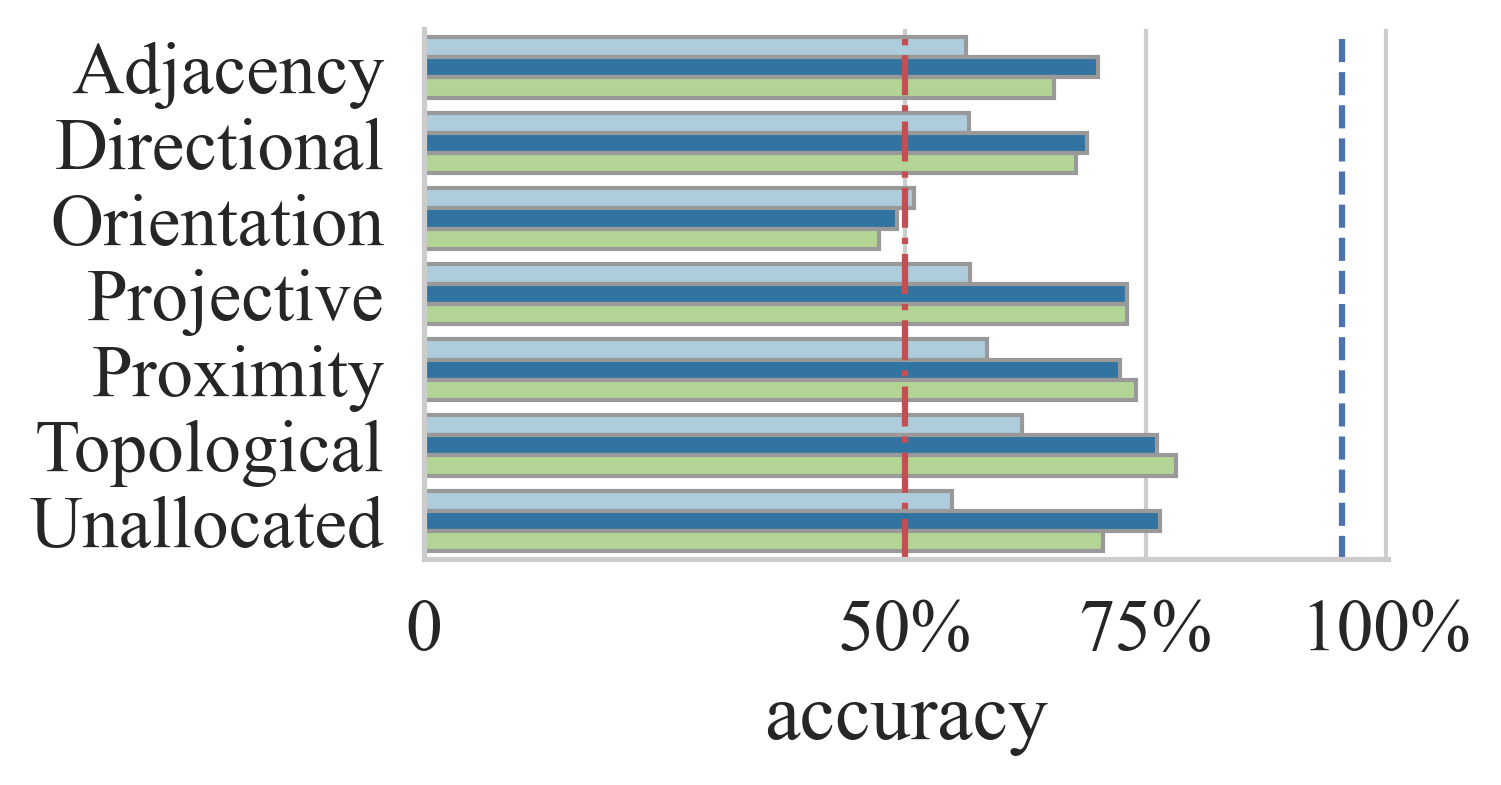
\includegraphics[width=\linewidth]{images/visual-spatial-reasoning/performance_by_meta_cat_random_split_v2.png}
    \caption{random split}
\end{subfigure}
\begin{subfigure}[b]{0.49\linewidth}
    \centering
    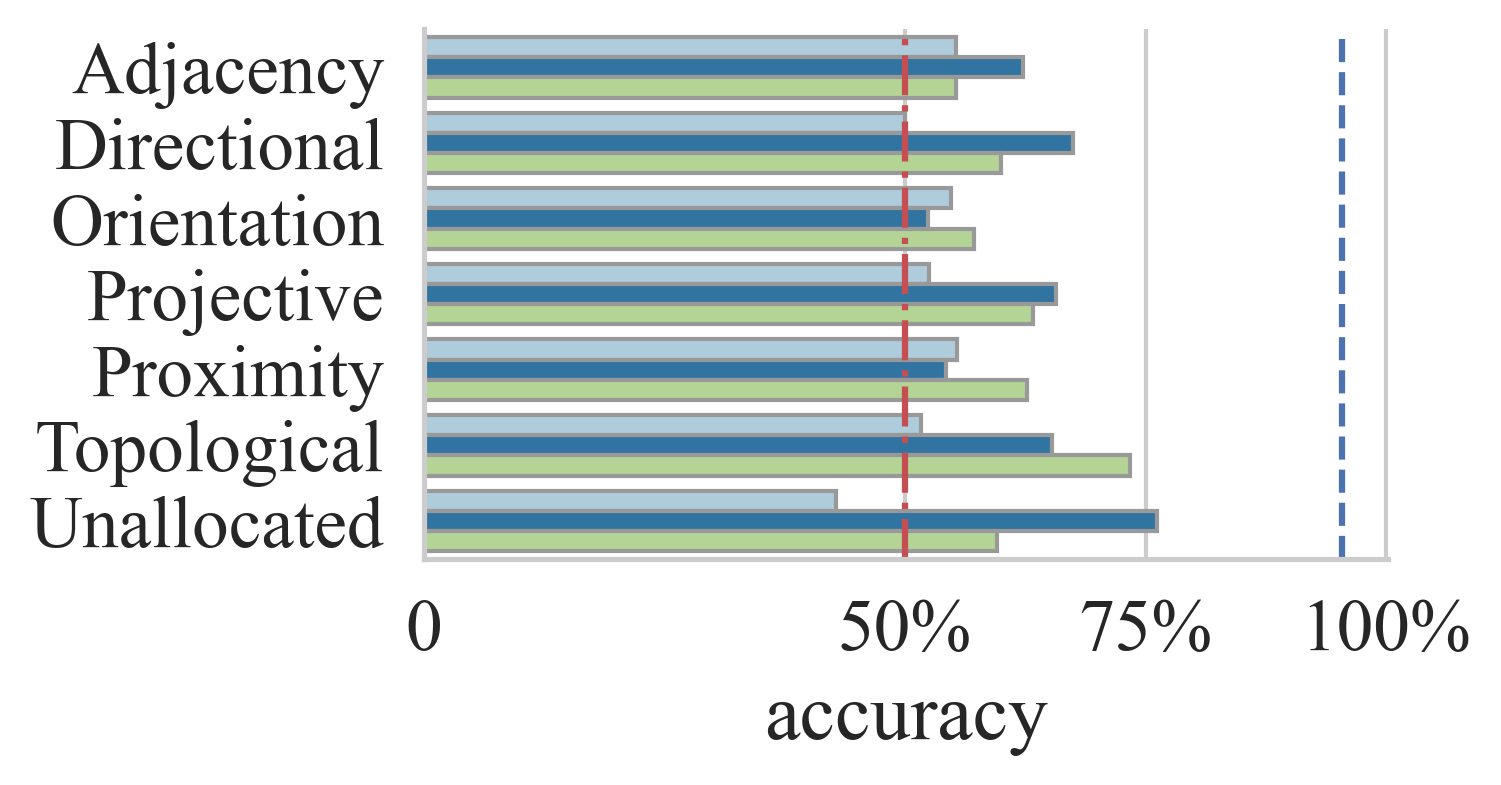
\includegraphics[width=\linewidth]{images/visual-spatial-reasoning/performance_by_meta_cat_zeroshot_split_v2.png}
    \caption{zero-shot split}
\end{subfigure}
\caption{Performance by meta categories of relations, on the random (left) and zero-shot (right) split test sets. For legend information, see \Cref{fig:performance_by_rel_base}.}
    \label{fig:performance_by_meta_cat_base}
\end{figure*}

\paragraph{Ours}

See \cref{fig:performance_by_meta_cat}

\begin{figure}[ht]
    \centering
    \begin{subfigure}[b]{0.49\linewidth}
    \centering
    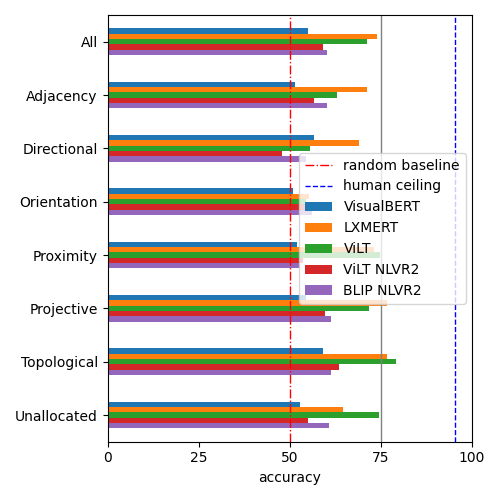
\includegraphics[width=\linewidth]{images/visual-spatial-reasoning/performance_rel_meta_cat_random.png}
    \caption{random split}
     \end{subfigure}
     \begin{subfigure}[b]{0.49\linewidth}
         \centering
    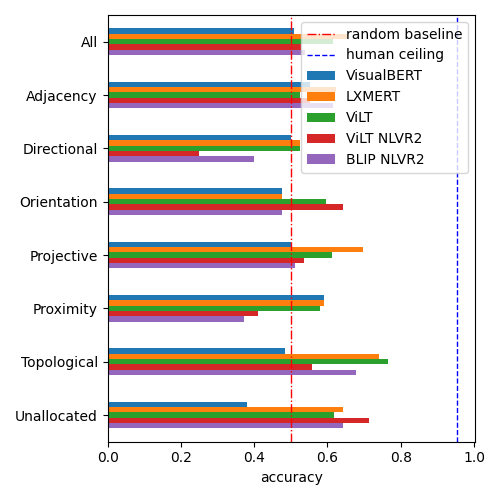
\includegraphics[width=\linewidth]{images/visual-spatial-reasoning/performance_rel_meta_cat_zeroshot.png}
         \caption{zero-shot split}
     \end{subfigure}
\caption{Performance by meta categories of relations, on the random (left) and zero-shot (right) split test sets. For legend information, see \cref{fig:performance_by_rel}.}
    \label{fig:performance_by_meta_cat}
\end{figure}

See \cref{tab:results-by-relation-meta-category-random} and \cref{tab:results-by-relation-meta-category-zeroshot}

\begin{table}[ht]
\centering
\begin{tabular}{lrrrrrr}
\toprule
category &  number &  VisualBERT &  LXMERT &  ViLT &  ViLT NLVR2 &  BLIP NLVR2 \\
\midrule
All         &    2024 &        55.1 &    73.9 &  71.2 &        59.1 &        60.1 \\
\midrule
Adjacency   &     284 &        51.4 &    71.1 &  63.0 &        56.7 &        60.2 \\
Directional &      90 &        56.7 &    68.9 &  55.6 &        47.8 &        54.4 \\
Orientation &     112 &        50.9 &    55.4 &  54.5 &        55.4 &        56.2 \\
Proximity   &     123 &        52.0 &    73.2 &  74.8 &        53.7 &        52.8 \\
Projective  &     773 &        54.5 &    76.7 &  71.7 &        59.8 &        61.4 \\
Topological &     591 &        59.2 &    76.8 &  79.2 &        63.5 &        61.4 \\
Unallocated &      51 &        52.9 &    64.7 &  74.5 &        54.9 &        60.8 \\
\bottomrule
\end{tabular}
\caption{Number and performance by relation meta category on the random split test.}
\label{tab:results-by-relation-meta-category-random}
\end{table}

\begin{table}[ht]
\centering
\begin{tabular}{lrrrrrr}
\toprule
category &  number &  VisualBERT &  LXMERT &  ViLT &  ViLT NLVR2 &  BLIP NLVR2 \\
\midrule
All         &     731 &        50.8 &    65.5 &  61.6 &        52.8 &        53.9 \\
\midrule
Adjacency   &     114 &        55.3 &    62.3 &  52.6 &        55.3 &        61.4 \\
Directional &      40 &        50.0 &    52.5 &  52.5 &        25.0 &        40.0 \\
Orientation &      42 &        47.6 &    47.6 &  59.5 &        64.3 &        47.6 \\
Proximity   &      83 &        59.0 &    59.0 &  57.8 &        41.0 &        37.3 \\
Projective  &     286 &        50.0 &    69.6 &  61.2 &        53.5 &        51.0 \\
Topological &     124 &        48.4 &    74.2 &  76.6 &        55.6 &        67.7 \\
Unallocated &      42 &        38.1 &    64.3 &  61.9 &        71.4 &        64.3 \\
\bottomrule
\end{tabular}
\caption{Number and performance by relation meta category on the zero-shot split test.}
\label{tab:results-by-relation-meta-category-zeroshot}
\end{table}
